\documentclass[10pt,oneside]{article}

\usepackage[T1]{fontenc}

\usepackage[paper=a4paper,margin=2cm,bottom=2.5cm]{geometry}
\usepackage[sfdefault,light,condensed]{roboto}
\usepackage[export]{adjustbox}
\usepackage[usenames,dvipsnames,table]{xcolor}

\usepackage{amsmath,amssymb,array,fancyhdr,graphicx,enumitem,lastpage,listings,lstautogobble,multicol,tabularx,textcomp,titlesec}
\usepackage{mathtools}

\setlength\parindent{0cm}
\renewcommand\headrule{}
\setlength{\footskip}{1.25cm}


\pagestyle{fancy}

\usepackage{fontawesome,subcaption,tikzsymbols}

% Add some padding to all table cells.
\setlength\extrarowheight{1pt}

%\newcommand{\boxwidth}{\dimexpr\linewidth - 2pt}
\newcommand{\boxwidth}{\linewidth}

\definecolor{BoxHeaderBG}{RGB}{50, 50, 50}
\definecolor{BoxHeaderText}{RGB}{220, 220, 220}

\definecolor{QuestionHeaderBG}{RGB}{200, 200, 200}
\definecolor{QuestionHeaderText}{RGB}{0, 0, 0}

\newcommand{\BoxHeader}[2]{
    \multicolumn{#1}{| >{\bfseries\footnotesize\cellcolor{BoxHeaderBG}\arraybackslash}l |}{
        \textcolor{BoxHeaderText}{#2}
    }
}

\newcounter{QuestionCounter}

\newcommand{\Question}[2]{
    \stepcounter{QuestionCounter}
    \begin{tabularx}{\boxwidth}{|X|}
        \hline
        \cellcolor{QuestionHeaderBG}{\footnotesize\bfseries \textcolor{QuestionHeaderText}{Question \#\theQuestionCounter}} {\em \textcolor{QuestionHeaderText}{#1}} \\\hline
        \ \\[#2]\hline
    \end{tabularx}

    \medskip
}

\newcommand{\FeelQuestion}{
    \stepcounter{QuestionCounter}
    \newcolumntype{F}{>{\centering\arraybackslash}X}
    \begin{tabularx}{\boxwidth}{| F F F |}
        \hline
        \multicolumn{3}{| >{\hsize=\dimexpr3\hsize+4\tabcolsep+2\arrayrulewidth\relax}X |}{
            \cellcolor{QuestionHeaderBG}{\footnotesize\bfseries \textcolor{QuestionHeaderText}{Question \#\theQuestionCounter}} {\em \textcolor{QuestionHeaderText}{Select the option which best reflects how confident you are in applying what you have learend in this lesson.}}}\\\hline
        & & \\[-8pt]
        \Sadey[5][orange] & \Neutrey[5][gray] & \Smiley[5][cyan] \\\hline
    \end{tabularx}

    \medskip
}

\lhead{\tiny\texttt{U\UnitNumber: \UnitTitle\\L\LessonNumber: \LessonTitle}}
\rhead{\tiny\texttt{[DPCS/\CourseLevel/U\UnitNumber/\LessonNumber]\\ }}

\lfoot{
\includegraphics[height=2cm,valign=c]{Files/logo}}
\cfoot{\footnotesize \LessonTitle/DPCS/\CourseLevel/U\UnitNumber/L\LessonNumber/\thepage/\pageref{LastPage}\\Woodstock School/Mussoorie, Uttarakhand, India}
\rfoot{
\includegraphics[height=2cm,valign=c]{Files/ib-world-school-logo-1-colour}}


\def\CourseLevel{SL}

\def\UnitNumber{01}
\def\UnitTitle{The Computer}

\def\LessonNumber{01}
\def\LessonTitle{Computer Architecture}

\begin{document}
    %Lesson Title
    \begin{center}
        \Large\bfseries \LessonTitle
    \end{center}

    % Objectives List
    \begin{tabularx}{\boxwidth}{|>{\small\raggedleft\bfseries\arraybackslash}p{0.1\textwidth} >{\small\arraybackslash}X |}
        \hline
        \BoxHeader{2}{Objectives} \\\hline
        2.1.1 & Outline the architecture of the central processing unit (CPU) and the functions of the arithmetic logic unit (ALU) and the control unit (CU) and the registers within the CPU. \\
        2.1.2 & Describe primary memory. \\
        2.1.3 & Explain the use of cache memory. \\
        2.1.5 & Identify the need for persistent storage. \\\hline
    \end{tabularx}

    % Opening Exercise
    \section*{Before You Begin}
    The following diagram represents a simple \emph{abstraction} of a computer system.

    \begin{figure}[h]
        \centering
        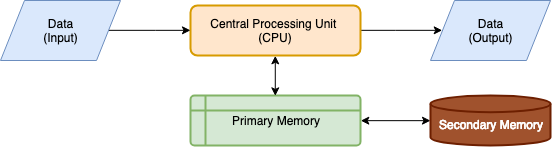
\includegraphics[width=0.75\boxwidth]{Extras/computer_abstraction_simple}
        \caption{A simple abstraction of a computer system.}
    \end{figure}

    Based on your own knowledge of computers, complete the following table with a brief description of each component. Include examples of computer hardware which would fulfill each role, where appropriate.

    \begin{tabularx}{\boxwidth}{| p{0.25\boxwidth} | X | p{0.25\boxwidth} |}
        \hline
        \BoxHeader{1}{Component} & \BoxHeader{1}{Description} & \BoxHeader{1}{Example} \\\hline
        Data (Input) & & \\[1cm]\hline
        Central Processing Unit (CPU) & & \\[1cm]\hline
        Primary Memory & & \\[1cm]\hline
        Secondary Memory & & \\[1cm]\hline
        Data (Output) & & \\[1cm]\hline
    \end{tabularx}

    \vfill

    \Question{A diagram such as the one above is a form of \emph{abstraction}. This abstraction hides the complexity of the specific inner workings of a computer system behind a simple flow diagram. Why do you think understanding abstractions such as these is important to the study of computer science?}{3cm}

    \pagebreak
    
    % Definitions
    \section*{Important Terms}
    \begin{tabularx}{\boxwidth}{| >{\bfseries\arraybackslash}p{0.3\boxwidth} | X | }
        \hline
        \BoxHeader{1}{Term} & \BoxHeader{1}{Definition} \\\hline
        Arithmetic Logic Unit (ALU) & \\[1.5cm]\hline
        Bus & \\[1.5cm]\hline
        Cache & \\[1.5cm]\hline
        Control Unit (CU) & \\[1.5cm]\hline
        Memory Unit (MU) & \\[1.5cm]\hline
        Random Access Memory (RAM) & \\[1.5cm]\hline
        Ready-Only Memory (ROM) & \\[1.5cm]\hline
        Register & \\[1.5cm]\hline
        \hspace{0.25cm} Memory Address Register & \\[1.5cm]\hline
        \hspace{0.25cm} Memory Data Register & \\[1.5cm]\hline
    \end{tabularx}

    \pagebreak

    % Technical Background
    \section*{Technical Background}

    \subsection*{Adding Complexity}
    The following diagram shows a more complete view of a computer system. Note the additional complexity outlined in the CPU and Primary Memory sections of the diagram.

    \begin{figure}[h]
        \centering
        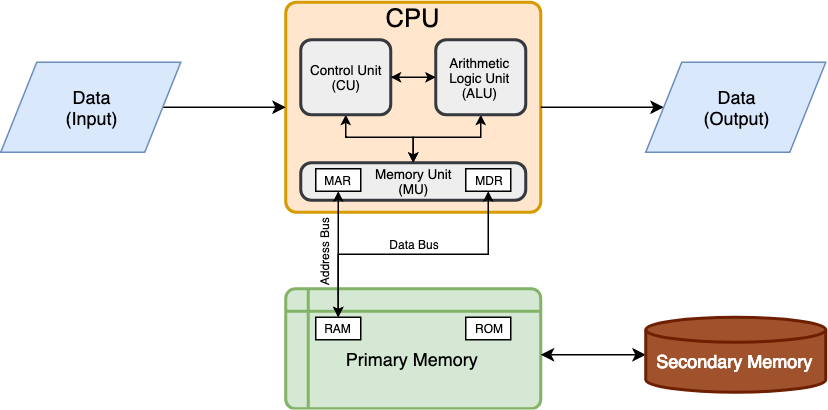
\includegraphics[width=0.75\boxwidth]{Extras/computer_abstraction_complex}
        \caption{Adding complexity by ``zooming in'' on the CPU and Primary Memory.}
    \end{figure}

    \subsubsection*{Notes}

    \vfill

    \Question{Although the above diagram has an increased level of complexity, it still represents only an abstraction of a computer system. Why might we want to represent the same system at different levels of abstraction?}{3cm}

    \Question{Secondary memory devices, such as traditional hard disk drives (HDDs) and solid-state drives (SSDs) are extremely common in computer systems. Briefly explain the need for these secondary memory devices. Are there any computer systems that might not require secondary memory?}{3cm}

    \pagebreak
    \subsection*{Even More Complexity}
    The following diagram represents the most complex abstraction of a computer system we will be discussing. It includes the L1/L2/etc. caches as part of the CPU.

    \begin{figure}[h]
        \centering
        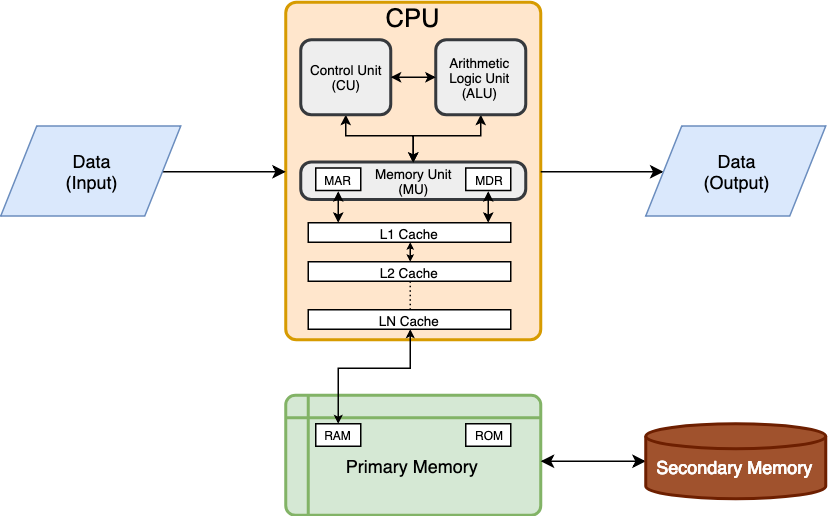
\includegraphics[width=0.75\boxwidth]{Extras/computer_abstraction_complex2}
        \caption{Adding even more complexity by examining the CPU's cache memory.}
    \end{figure}

    \subsubsection*{Notes}

    \vfill
    
    \Question{Modern processors often include many different ``levels'' of caches, numbered according to their ``closeness'' to the main control unit. What impact do you think this has on the performance of the computer system? Why do you think different levels of caches are used rather than increasing the size of a single cache?}{4cm}

    \pagebreak
    
    % Developing Technical Skills
    \section*{Developing Technical Skills}
    \subsubsection*{Examining Computer Specifications}

    Use the following steps to discover system information about your personal computer.

    \begin{tabularx}{\boxwidth}{| X | X |}
        \hline
        \BoxHeader{1}{Windows (7/8/10)} & \BoxHeader{1}{Mac OSX} \\\hline
        {
            \begin{enumerate}[noitemsep]
                \item Press \faWindows\ + r.
                \item Type ``msinfo32'' and hit enter.
            \end{enumerate}
        } &
        {
            \begin{enumerate}[noitemsep]
                \item Click the \faApple\ logo.
                \item Hold the option key and select ``System Information''.
            \end{enumerate}
        }
        \\\hline
    \end{tabularx}
    
    \medskip
    Using the information provided by your operating system, as well as supplemental information from online sources, fill out the following information about your system.

    \begin{tabularx}{\boxwidth}{| p{0.3\boxwidth} | X |}
        \hline
        \BoxHeader{1}{Component} & \BoxHeader{1}{Description} \\\hline
        \BoxHeader{2}{Processor} \\\hline
        Model & \\[0.75cm]\hline
        Speed & \\[0.75cm]\hline
        Cores & \\[0.75cm]\hline
        Caches & \\[0.75cm]\hline
        \hspace{0.25cm} Cache Size (L1) & \\[0.75cm]\hline
        \hspace{0.25cm} Cache Size (L2) & \\[0.75cm]\hline
        \hspace{0.25cm} Cache Size (L3) & \\[0.75cm]\hline
        \BoxHeader{2}{Memory} \\\hline
        Ram & \\[0.75cm]\hline
        Secondary Memory (HDD/SDD) & \\[0.75cm]\hline
    \end{tabularx}

    \vfill

    \Question{Why do you believe computer systems vary as much as they do? What impact does this variance have on the computer industry as a whole?}{4cm}

    \pagebreak

    % Reflections
    \section*{Reflections}

    \Question{Why is it important for computer scientists to have some knowledge of a computer's inner workings?}{4cm}

    \Question{Why do you think we have no tincluded specific input and output devices in our abstract models of a computer system?}{4cm}

    \Question{Describe at least one new thing you have learned from this lesson. How might you apply this knowledge in the future?}{4cm}

    \FeelQuestion

    \Question{What further questions do you still have about this lesson's content?}{4cm}
\end{document}